\documentclass[prb,showpacs,amssymb,amsmath,twocolumn]{revtex4-1}
%%%%%%%%%%%%
\usepackage{bookmath} % definitions and shortcuts
%%%%%%%%%%%%
%\usepackage{fullpage}
\usepackage{graphicx}
\usepackage[justification=justified,singlelinecheck=false,font=small,format=plain,labelfont=bf,up,textfont=normal,up]{caption}
\usepackage{subcaption}
%\usepackage{wrapfig}
\usepackage{amsmath}
\usepackage{anyfontsize}
\usepackage{color}
\newcommand{\blue}{\textcolor{blue}}
\newcommand{\red}{\textcolor{red}}
\newcommand{\cecoin}{CeCoIn$_5$} 




%~~~~~~~~~~~~~~~~~~~~~~~~~~~~~~~~~~~~~~~~~~~~~~~~~~~~~~~~~~~~~~~~~~~~~~~~~~~~~~~%
\begin{document}
%~~~~~~~~~~~~~~~~~~~~~~~~~~~~~~~~~~~~~~~~~~~~~~~~~~~~~~~~~~~~~~~~~~~~~~~~~~~~~~~%
\title{Electronic Spin Susceptibility Enhancement in Pauli Limited Unconventional Superconductors}

\author{Ben Rosemeyer, Anton Vorontsov}

\affiliation{Department of Physics, Montana State University, Montana 59717, USA}

\date{\today}

\begin{abstract}
%
We calculate the wave-vector dependent electronic spin susceptibility 
$\chi_{\alpha\beta}(\vq, \vH_0)$ 
of a superconducting state in uniform magnetic field $\vH_0$. 
We consider Pauli limited materials with $d$-wave symmetry, and a 2D cylindrical 
electronic Fermi surface.  
We find that both longitudinal and transverse components of the susceptibility tensor are enhanced over their
normal state values in the high-field low-temperature region of the $H-T$
phase diagram. We identify several wave vectors, connecting field-produced hot spots on the Fermi surface, 
that correspond to the enhancement of either $\chi_\perp$ or $\chi_\parallel$ components. 
%
\end{abstract} 

\pacs{74.20.Rp,74.25.Dw, \red{MORE?,DIFFERENT?} }

%74.20.Rp 	Pairing symmetries (other than s-wave) 
%74.25.Dw 	Superconductivity phase diagrams 


\maketitle



%~~~~~~~~~~~~~~~~~~~~~~~~~~~~~~~~~~~~~
\section{Introduction}
%~~~~~~~~~~~~~~~~~~~~~~~~~~~~~~~~~~~~~
%
The interplay of different orders, simultaneously present in the same system, 
is of a great interest to physics community and beyond. 
Such interactions present another level of complexity in emergent systems. 
They offer insight into the properties of the ordered phases, but also 
often pose a great challenge both mathematically 
and conceptionally.\cite{x}\red{not sure what to cite here...} 
The two most widely studied orders, that often appear together in many systems, 
are superconductivity and magnetism, both having their origin tightly 
connected to the behavior of the quantum mechanical spin. 
The behavior of these orders have been investigated under many different conditions. 
Ferromagnetic order and singlet superconductivity avoid each other since they have opposite spin 
structures\cite{x}; 
on the contrary triplet superconductivity is much less sensitive to the ferromagnetism\cite{x}; 
antiferromagnetic order with spatial period much smaller than the superconducting coherence length 
does not interfere with superconductivity, and the two orders may easily appear together\cite{x},  
and in some cases unconventional superconducting and spin-density wave orders even attract each other\cite{x}. 

Despite this great amount of knowledge, the 
interplay of antiferromagnetism (AFM) and superconductivity (SC) still often challenges
our understanding of this phenomenon, for various reasons. 
For example, materials such as cuprate oxides have unusual normal state properties \cite{x}, 
whereas iron-based superconductors have complex orbital multiband structure\cite{x}. 

%%%%%%%%%%%%%%%%%%%%%%%%%%%%%%%%%%%%%%%%%%%%%%%%%%%%%%%%%%%%%%%%%%%%%%%%%%%%%%%%%
\begin{figure}
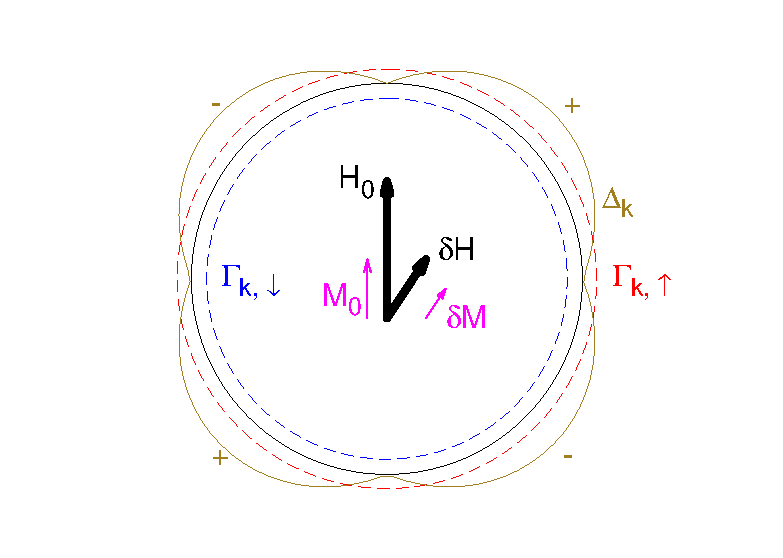
\includegraphics[height = 0.4\textwidth, width = 0.4\textwidth]{./figures/fermi_schematic.eps}
\caption{\begin{flushleft}
We consider 2D electrons with circular Fermi surface (FS). 
Zeeman interaction splits Fermi surfaces for up and down spins ($\Gamma_{\vk \uparrow}, \Gamma_{\vk \downarrow}$). 
The $d$-wave order parameter $\Delta_\vk \propto \sin 2\theta_\vk $ is also shown. 
Magnetic field produces pockets of low energy spin-down excitations near the nodes of the order parameter. \end{flushleft}
\label{fig:FS}
}
\end{figure}
%%%%%%%%%%%%%%%%%%%%%%%%%%%%%%%%%%%%%%%%%%%%%%%%%%%%%%%%%%%%%%%%%%%%%%%%%%%%%%%%%

One other, interesting and relatively recent example, is heavy-fermion material 
\cecoin, which manifests a coexistent AFM and superconducting state (Q-phase) \cite{cecoin5_Bianchi, cecoin5_Kenzelmann, cecoin5_Kenzelmann2}
in the high-field low-temperature limit. 
Experimental results for \cecoin\ indicate that this co-existence is the result of 
strong attraction between superconducting unconventional $d$-wave order, 
and the AFM state\cite{cecoin5_Bianchi,cecoin5_Kenzelmann,cecoin5_Kenzelmann2}. 
The Q-phase and magnetism disappear when superconductivity is suppressed at the upper critical field $H_{c2}$ 
through a first order transition to the normal state. 
The magnetic order appears inside the SC state through a second order transition. 
Moreover, although the normal state of \cecoin\ is non-magnetic, the proximity to magnetic 
instability can be demonstrated by applying doping to induce it, or pressure, to destroy it.\cite{doped_cecoin5, cecoin5_Kenzelmann, cecoin5_Kenzelmann2, cecoin5_magnetism_chapter} 

\red{To be edited more...} 

Other results for \cecoin\ show that the magnetic ordering wave vector in the
Q-phase displays little or no dependence on field (within experimental error),
which indicates a relatively small or non-existent interaction with the flux
lattice \cite{cecoin5_Kenzelmann2}. This phenomenon has not been directly
addressed in many of the current theories. Our findings indicate that this
behavior is more consistent with the longitudinal component of suscep	tibility
rather than the transverse. This is another area of study which has not been
very thouroghly analyzed.

Many theories have been proposed to explain the experimental results seen in
\cecoin, including various manifestations of the FFLO state where the
superconducting order parameter oscillates in real space.
\cite{sc_sdw_anton,mag_afm_fflo_sigrist,fflo_pen_depth,sc_afm_kato,sc_afm_ikeda,sdw_vortex}.
The FFLO state has long been believed to offer the possibility of magentic
order, however, the predicted field dependence of the ordering vector is not
seen in experiment, and recent experiments point to a homogeneous gap function
\cite{cecoin5_Kenzelmann2,cooperPairsCeCoIn5}.

Yet other theories offer insight but leave many questions unanswered. Such as:
How does the ordering wave vector change with applied field? What are the
necessary conditions on the order parameter? And what roles do the transverse
and longitudinal components of the magnatism play? Here we provide a first
principles approach to these problems by calculating the magnetic
susceptibility of itinerant electrons in the D-wave superconducting state. 
In this paper we investigate the microscopic underlay of such interaction. 





%~~~~~~~~~~~~~~~~~~~~~~~~~~~~~~~~~~~~~
\section{Model}
%~~~~~~~~~~~~~~~~~~~~~~~~~~~~~~~~~~~~~
%
To investigate the interplay of superconductivity and magnetic order in external field,  
we consider mean-field SC Hamiltonian of 2D electrons with cylindrical FS, interacting with magnetic field 
through Zeeman term: 
\bea
\cH = \cH_{N} + \cH_{sc} + \cH_{Z} \\ \label{eq:modelH}
\cH_{N} = \sum_{\vk,\mu} \xi_\vk c_{\vk,\mu}^\dag c_{\vk,\mu}\nonumber   \\
\cH_{sc} = \sum_\vk \left( \Delta_\vk c_{\vk,\uparrow}^\dag c_{-\vk,\downarrow}^\dag + h.c. \right)\nonumber  \\
\cH_Z(\vH) = \sum_{\vk,\mu,\nu} c_{\vk_+\vq,\mu}^\dag  \mu_B \vsigma_{\mu\nu} (\vH_0 \delta_{\vq,0} + \delta\vH_\vq) c_{\vk,\nu}  
\nonumber 
\eea
where the electronic dispersion in the normal state is $\xi_{\vk}=\frac{\vk^2}{2m^*}-\epsilon_F$, 
and $\mu_B$ is the magnetic moment of electron (Bohr magneton). 
We assumed a strong uniform magnetic field and perturbation at wavevector $\vq$, 
\be
\vH(\vR) = \vH_0 + \delta \vH_\vq e^{i\vq \cdot \vR} \,.
\ee
The resulting magnetization is due to the interaction term $V = -\vm \cdot \vH$, and also has uniform part and linear response to perturbation:
\bea
M_\alpha(\vR) = M_{0\alpha}(\vH_0) + \delta M_\alpha(\vR)
\\
\delta M_\alpha(\vR) = \chi_{\alpha\beta} (\vq) \delta H_\beta e^{i\vq \cdot \vR}
\eea
given by the standard expressions.\cite{mahan} 
\begin{widetext}
\bea
\mbox{\red{Add equation for }} \vM_0\,,  \mbox{\red{ Check expression for }} \chi\,, \mbox{\red{ Check transformation}}
\\
M_{\alpha}(t) = -i \int \limits_{-\infty}^t <[m_\alpha(t) , V(t')]>_{_0} dt' \\
\chi_{\alpha\beta}(\vx,\vx', \omega)=-i \mu_B^2\sum\limits_{\mu\mu'\nu\nu'}\int\limits_{-\infty}^{0}dt' \; \sigma^\alpha_{\mu\mu'}\sigma^\beta_{\nu\nu'}e^{i\omega t'} \; 
\langle [\psi^\dagger_\mu(\vx ',t') \psi_{\mu'}(\vx ',t'),  \psi^\dagger_\nu(\vx,0) \psi_{\nu'}(\vx,0) ]\rangle_{_0}
\label{eq:susdef}
\eea
\end{widetext}
Where the subscript 0 on the average indicates the average over eigenstates of eq \ref{eq:modelH} with $\vH = \vH_0$.

We are mostly interested in the electronic susceptibility $\chi$, since it determines the magnetic instability into 
an SDW (spin-density wave) state, 
or responsible for RKKY-type interaction between localized moments on Ce atoms. 
To calculate the susceptibility (\ref{eq:susdef}) in superconducting state, we diagonalize 
the Hamiltonian (\ref{eq:modelH}) by the 
Bogoliubov transformation~\cite{tinkham}, 
that defines the elctron operators $c_{\vk \alpha}$ through 
new quasiparticle operators $\gamma_{\vk \alpha}$:


\bea
c_{\vk \mu} = u_\vk \gamma_{\vk \mu} + \sum\limits_{\mu'}(i\sigma_2)_{\mu\mu'} v_\vk^* \gamma^\dag_{-\vk \mu'}\\
\epsilon_{\vk,\mu}=\sqrt{\Delta_{\vk}^2+\xi_{\vk}^2} + (\sigma_3)_{\mu\mu}\mu_B H_0 \\
u_{\vk}=\sqrt{\frac{1}{2}\left( 1+\frac{\xi_{\vk}}{\sqrt{\Delta_{\vk}^2+\xi_{\vk}^2}} \right)} \\
v_{\vk}= \sgn(\Delta_\vk) \sqrt{\frac{1}{2}\left( 1-\frac{\xi_{\vk}}{\sqrt{\Delta_{\vk}^2+\xi_{\vk}^2}} \right)}
\eea

The diagonalized Hamiltonian is 
\be 
\cH = \sum_{\vk s} \epsilon_{\vk s} \gamma^\dag_{\vk s} \gamma_{\vk s} 
\ee 


We then use this Hamiltonian and time-dependent operators to compute the magnetic susceptibility of electrons. 
In the presence of external magnetic field $\vH_0$ the spin-rotational symmetry is broken even in magnetically 
isotropic system. 
Now one has to distinguish between two possibilities for the direction of the wave-vector dependent magnetization: 
(a) $\delta \vM(\vq) \parallel \vH_0$ (longitudinal response), and 
(b) $\delta \vM(\vq) \perp \vH_0$ (transverse response). 
In standard literature e.g.\cite{x}\red{book?} it is discussed that the longitudinal response is usually smaller than the transverse, 
in case of antiferromagnetism. 
We will show, however, that the standard reasoning is not applicable here, where the magnetic field and presense 
of unconventional superconductivity create a new environment/terms in GL functional that stabilize the parallel 
component as well. 
%%%%%%%%%%%%%%%%%%%%%%%%%%%%%%%%%%%%%%%%%%%%%%%%%%%%%%%%%%%%%%%%%%%%%%%%%%%%%%%%%
\begin{figure}
 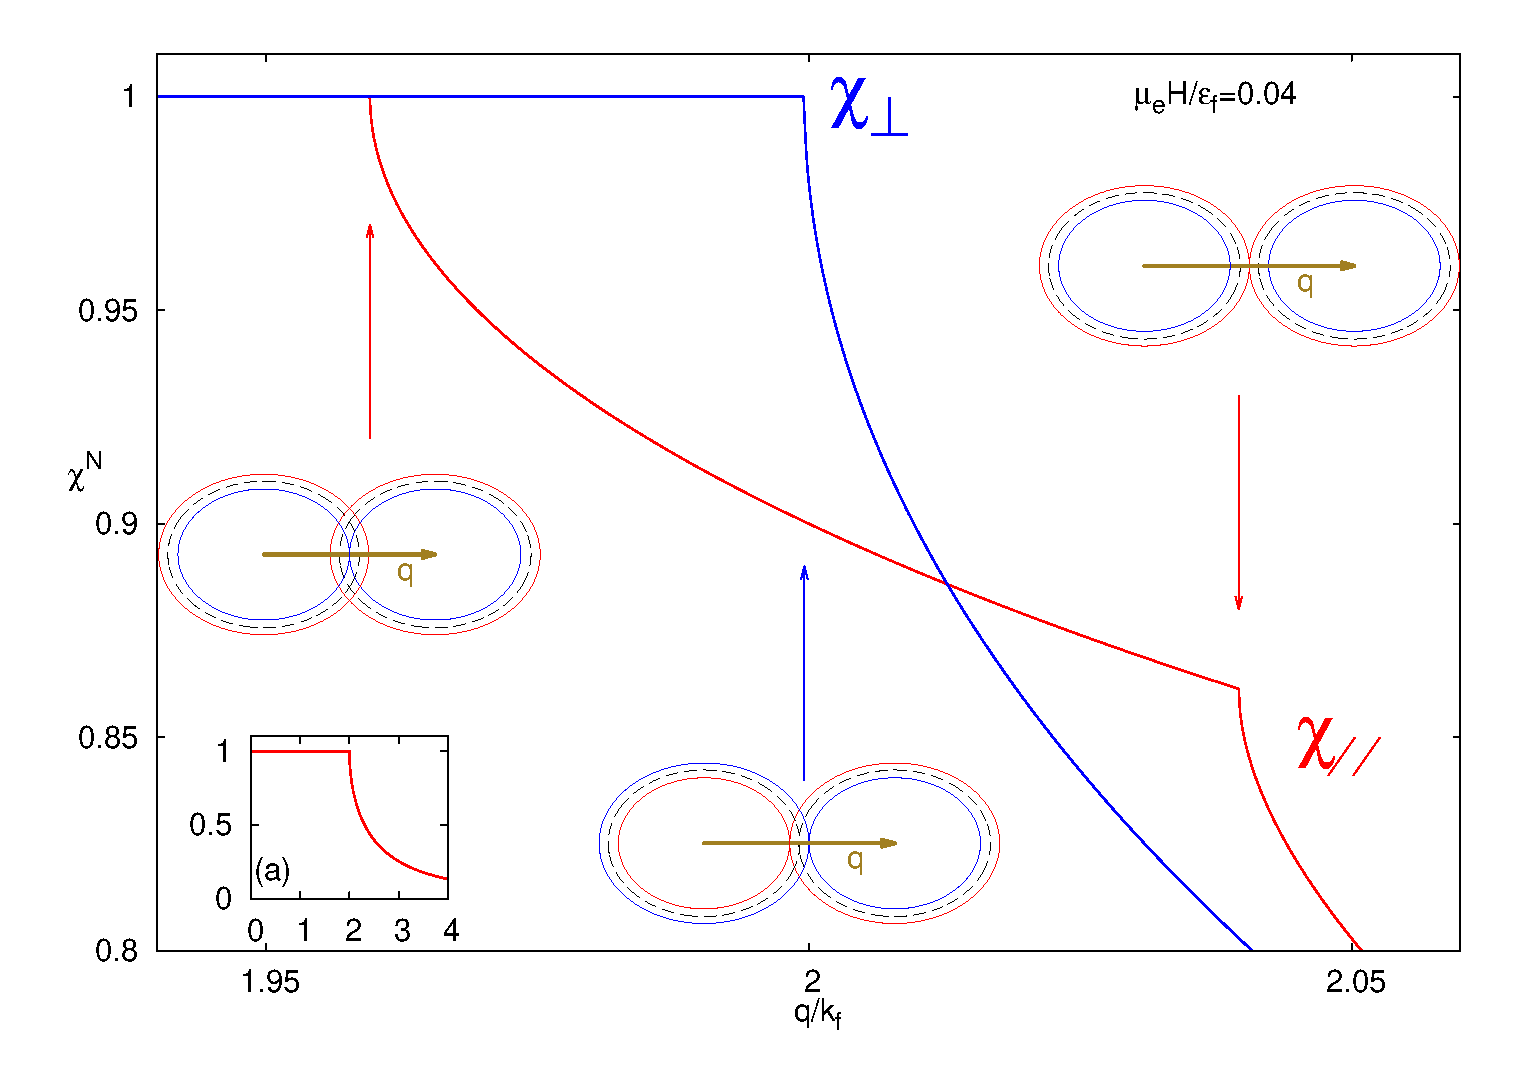
\includegraphics[width=0.45\textwidth, height=0.45\textwidth]{./figures/normal_chi_spin_pairing_.eps}
 \caption{\begin{flushleft}The 2D normal state susceptibility in zero field has a discontinuity in the first derivative for $q=2k_f$ (a). Including Zeeman interaction, the location of these depend on the applied field and how the spins are paired for the different components (insets). The longitudinal component pairs equal spins so there are two discontinuities ($q_\pm = 2\sqrt{\epsilon_f \pm \mu_B H_0}$), while the transverse component pairs opposite spins leading to only one discontinuity ($q = \sqrt{\epsilon_f + \mu_B H_0} + \sqrt{\epsilon_f - \mu_B H_0}$)\end{flushleft}
 \label{fig:norm}
 }
 \end{figure}
 %%%%%%%%%%%%%%%%%%%%%%%%%%%%%%%%%%%%%%%%%%%%%%%%%%%%%%%%%%%%%%%%%%%%%%%%%%%%%%%%%


The general expressions for the real part of the longitudinal and transverse susceptibilities are:\cite{spin_sus} 

\begin{widetext}
\bea
\label{eq:xi}
\chi^{sc}_{\parallel}({\bf q})=-\mu_B^2\sum\limits_{\vk,\mu} 
\frac{(f(\epsilon_{\vk_-\mu})-f(\epsilon_{\vk_+\mu}))(u_{\vk_+}u_{\vk_-}+v_{\vk_+}v_{\vk_-})^2}{\epsilon_{\vk_-\mu}-\epsilon_{\vk_+\mu}} 
-\frac{(1-f(\epsilon_{\vk_-\mu})-f(\epsilon_{\vk_+\bar{\mu}}))(u_{\vk_+}v_{\vk_-}-v_{\vk_+}u_{\vk_-})^2}{\epsilon_{\vk_-\mu}+\epsilon_{\vk_+\bar{\mu}}}
\\
\chi^{sc}_{\perp}({\bf q})=-\mu_B^2\sum\limits_{\vk,\mu} 
\frac{(f(\epsilon_{\vk_-\mu})-f(\epsilon_{\vk_+\bar{\mu}}))(u_{\vk_+}u_{\vk_-}+v_{\vk_+}v_{\vk_-})^2}{\epsilon_{\vk_-\mu}-\epsilon_{\vk_+\bar{\mu}}} 
-\frac{(1-f(\epsilon_{\vk_-\mu})-f(\epsilon_{\vk_+\mu}))(u_{\vk_+}v_{\vk_-}-v_{\vk_+}u_{\vk_-})^2}{\epsilon_{\vk_-\mu}+\epsilon_{\vk_+\mu}} \nonumber
\eea
\end{widetext}


where $\chi_0 = 2 \mu_B^2 N_F$ is Pauli susceptibility in the normal state, 
$f(\epsilon) = (\exp(\epsilon/T)+1)^{-1}$ is the Fermi distribution, 
and momenta are shifted by the magnetization wave vector $\vk_\pm = \vk \pm \vq/2$. The derivation of this result is presented in Appendix \ref{sec:appA}.



\section{Normal State}

We first review the results for the normal state susceptibility in magnetic field.  
By setting $\Delta_\vk = 0 $ in the general expression above, one obtains the familiar 
Lindhard function,  
\bea
\chi_{\parallel}=-2\mu_B^2\sum\limits_{\vk,\mu} \frac{
	f(\xi_{\vk,\mu})-f(\xi_{\vk_+\vq,\mu})}
	{\xi_{\vk,\mu}-\xi_{\vk_+\vq,\mu}} 
		\\
\chi_{\perp}=-2\mu_B^2\sum\limits_{\vk,s} \frac{
f(\xi_{\vk,\mu})-f(\xi_{{\bf \vk_+q},-\mu})}{
	\xi_{\vk,\mu}-\xi_{{\bf \vk_+q},-\mu}}  \nonumber
\eea
where $\xi_{\vk \mu} = \frac{k^2}{2m^*}-\epsilon_f + (\sigma_3)_{\mu\mu}\mu_B H_0$ are electron excitation 
energies in magnetic field 
(excluding orbital effects) 

At zero temperature the Fermi functions are step-functions, 
and the summation over momenta can be done analytically; 
in two dimensions we get (details of the integration is presented in appendix \ref{sec:appB}), 

\begin{widetext}
\bea
\frac{\chi^N_\parallel(q)}{\chi^N_0}& = 1-\frac{\Theta(q-2 k_{f\uparrow})}{2}\sqrt{1-(\frac{2}{q})^2k_{f\uparrow}^2}-\frac{\Theta(q-2k_{f\downarrow})}{2}\sqrt{1-(\frac{2}{q})^2k_{f\downarrow}^2}
   \\
\frac{\chi^N_\perp(q)}{\chi^N_0} &= 1-\Theta(q-k_{f\uparrow}-k_{f\downarrow})\sqrt{1-(\frac{2}{q})^2(1-(k_{f\uparrow}^2-k_{f\downarrow}^2)^2/(2q)^2)} 
\eea
\end{widetext}

%\red{\bf Maybe it would be better to talk of the phase space in the superconducting state. This is just an integral and is in the appendix.} 
%Where $=$
%The resulting equation(s) 5 have a discontinuity in the first derivitive (Interestingly, the 1D and 3D calculations have discontinuities in the 0th and 2nd derivitive respectively)~\cite{lindhard_fnct}. the
%origin of this is the competition between the amount of phase space available
%to the sum which is defined by the fermi functions, and the term in the
%denominator, which is proportional to the distance from the origin. For
%$q<2k_f$ these two balance each other perfectly (as q grows the available phase
%space grows and the average distance from the origin also increases). For
%$q>2k_f$ the amount of phase space available is maximized so it can no longer
%keep up with the average distance from the origin increasing, so the
%susceptibility begins to fall off. 
Where we have normalized everything so that $\epsilon_f = 1$ and $k_{f\uparrow\downarrow} ^2= 1\pm \mu_B H_0/\epsilon_f$.

When a field is applied to the system the transverse and longitudinal
components begin to differentiate themselves due to the way they connect spins
(fig. \ref{fig:norm}). The transverse component connects opposite spins so there is only one
critical q at which the paired surfaces touch each other at one point, 
$q=k_{f\uparrow} + k_{f\downarrow}$. The longitudinal component connects equal spins so there are
two critical q's at which the surfaces touch each other $q_{\uparrow} = 2k_{f\uparrow}$ and $q_\downarrow = 2k_{f\downarrow} $~\cite{lindhard_fnct}.


%~~~~~~~~~~~~~~~~~~~~~~~~~~~~~~~~~~~~~
\section{Superconducting State}
%~~~~~~~~~~~~~~~~~~~~~~~~~~~~~~~~~~~~~
%
We proceed further into the superconducting state with D-wave symmetry. The
inclusion of a Zeeman term in the superconducting Hamiltonian and a nodal order
parameter ensures that for high enough fields the Zeeman splitting of the
energy levels is enough to overcome the superconducting gap somewhere on the
Fermi surface. Resulting in quasi-particle hole states with negative energy $\epsilon_{\vk,\mu}<0$

Consequently, the $\epsilon_{\vk,\mu}=0$ contour (fig. \ref{fig:qq}) defines the region inside which $\epsilon_{\vk,2}<0$, and $f(\epsilon_{\vk,2}) = 1$. Only quasi particles with $\mu = 2$ provide this necessary condition which dictates the terms in equations \ref{eq:xi} that provide the major
contributions.

  %%%%%%%%%%%%%%%%%%%%%%%%%%%%%%%%%%%%%%%%%%%%%%%%%%%%%%%%%%%%%%%%%%%%%%%%%%%%%%%%%
  \begin{figure}
        \centering
                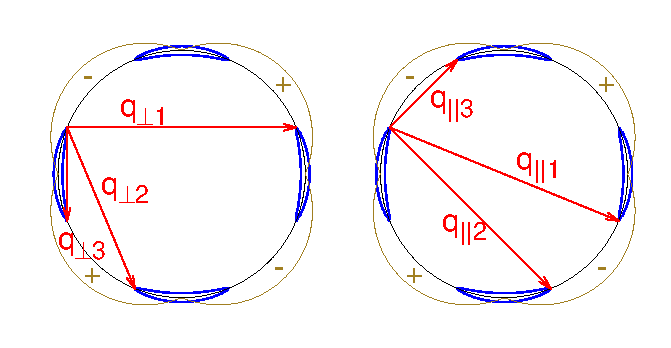
\includegraphics[scale=0.85]{./figures/Bananas_with_q.eps}
        \caption{\begin{flushleft} The critical wave vectors which connect points on the Fermi surface that have zero quasi-particle excitations for transverse and longitudinal afm. The blue outlines the region inside which $\epsilon_{\vk,2}<0$, while the olive is a schematic of the order parameter.\end{flushleft}
       \label{fig:qq}
        }
 \end{figure}
%%%%%%%%%%%%%%%%%%%%%%%%%%%%%%%%%%%%%%%%%%%%%%%%%%%%%%%%%%%%%%%%%%%%%%%%%%%%%%%%%



%%%%%%%%%%%%%%%%%%%%%%%%%%%%%%%%%%%%%%%%%%%%%%%%%%%%%%%%%%%%%%%%%%%%%%%%%%%%%%%%%
\begin{figure}
	
        \centering
                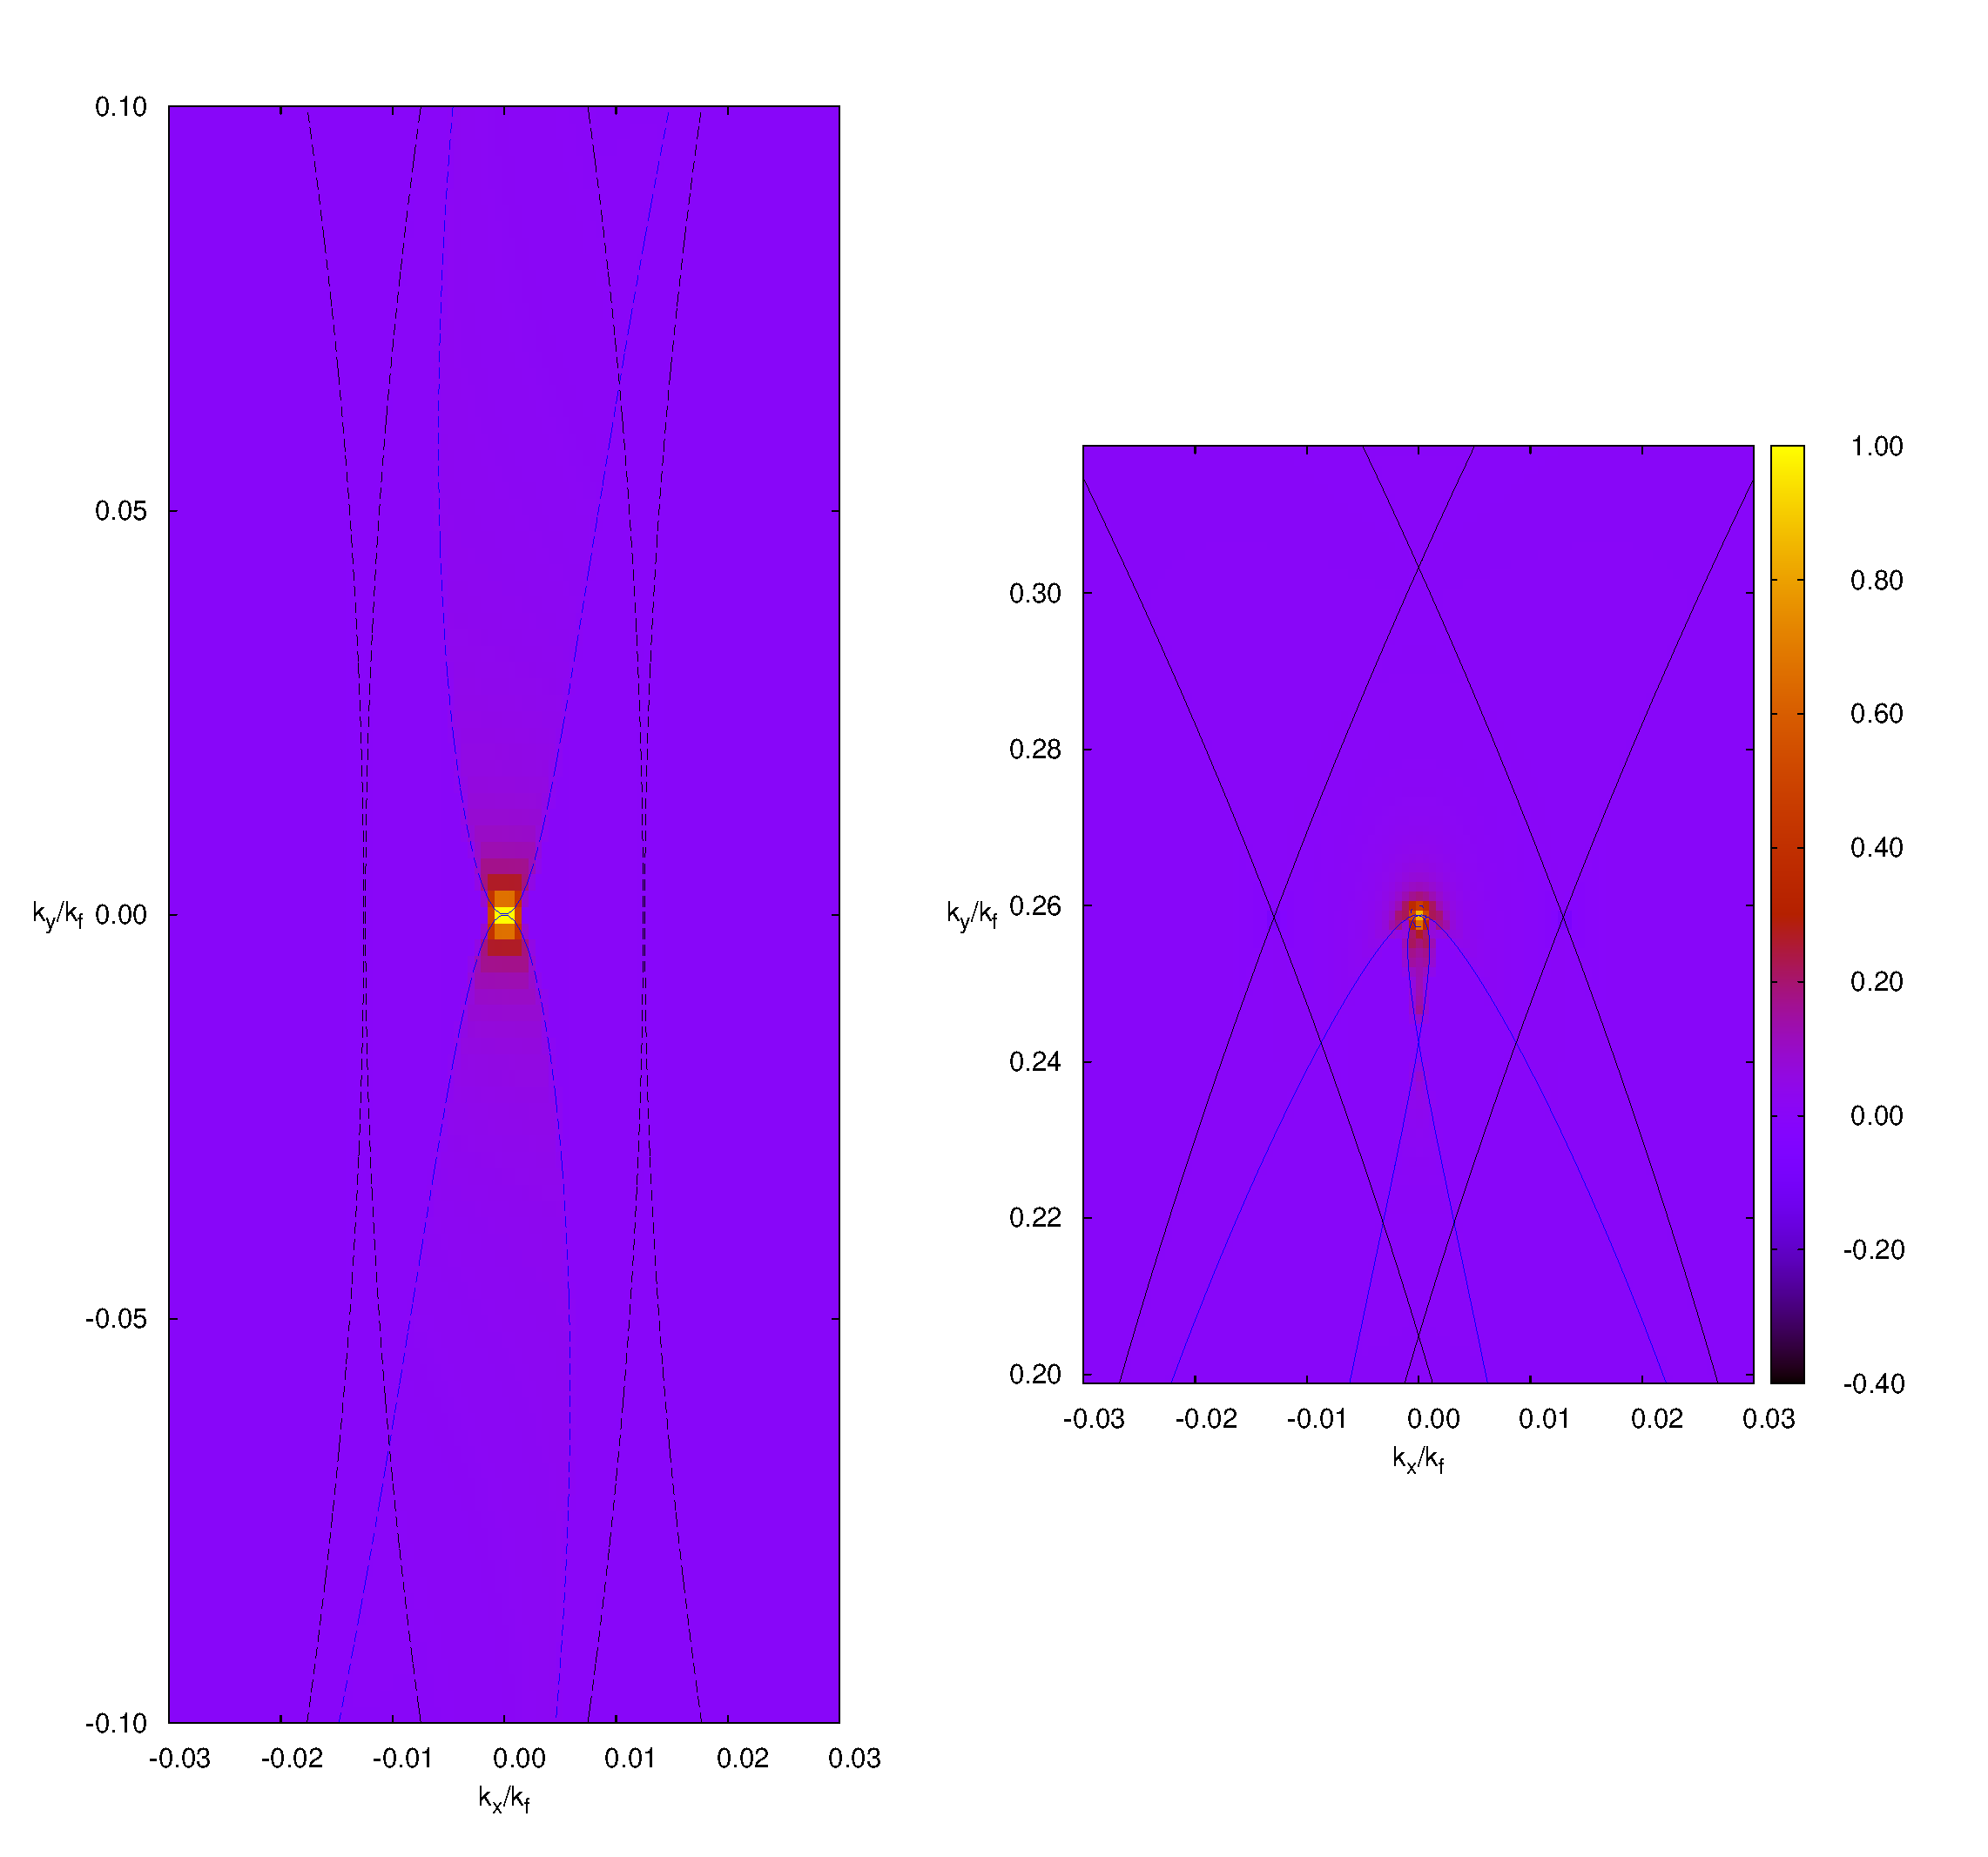
\includegraphics[scale = 0.2]{./figures/integrands.eps}
                \caption{\begin{flushleft}The $\delta\chi$ integrand for the longitudinal (left) and transverse (right) component at zero temperature and for $\vq_{\parallel 1}$ and $\vq_{\perp 1}$. The black lines are the Zeeman split fermi surfaces for normal electrons and the blue lines are the pockets inside which there are negative quasi-particle excitations.\end{flushleft} \label{fig:integrand}}


 \end{figure}
%%%%%%%%%%%%%%%%%%%%%%%%%%%%%%%%%%%%%%%%%%%%%%%%%%%%%%%%%%%%%%%%%%%%%%%%%%%%%%%%%
Analysis of the integrand for $\delta \chi_{\alpha}(\vq)=
\chi^{sc}_{\alpha}(\vq)- \chi^N_{\alpha}(\vq)$ indicates that value of
is less than $(\Delta_{00}/\epsilon_f)^2$ in the majority of phase space and
that the main contributions come from regions which are close to the
intersections of the two fermi surfaces (fig. \ref{fig:integrand}).~\cite{sc_afm_kato,sdw_vortex,sc_afm_ikeda}  
%~~~~~~~~~~~~~~~~~~~~~~~~~~~~~~~~~~~~~
\section{Discussion}
%~~~~~~~~~~~~~~~~~~~~~~~~~~~~~~~~~~~~~
%
 %%%%%%%%%%%%%%%%%%%%%%%%%%%%%%%%%%%%%%%%%%%%%%%%%%%%%%%%%%%%%%%%%%%%%%%%%%%%%%%%%
 \begin{figure}
        \centering
                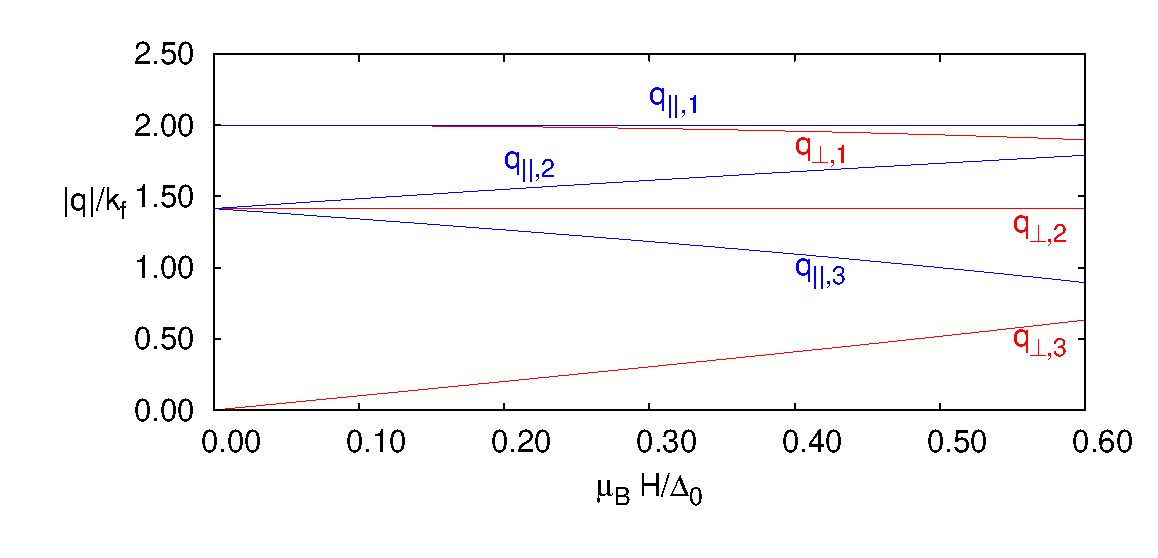
\includegraphics[width=0.45\textwidth]{./figures/qq_theory.eps}
                \caption{\begin{flushleft} The critical $\vq$'s shown in figure \ref{fig:qq} depend on the field. \end{flushleft}\label{fig:qqTheory}}

 \end{figure}
 %%%%%%%%%%%%%%%%%%%%%%%%%%%%%%%%%%%%%%%%%%%%%%%%%%%%%%%%%%%%%%%%%%%%%%%%%%%%%%%%%
We further search for the conditions on the wave vector for which $\chi^{sc}$ is
maximized. This occurs for ${\bf q}$'s which connect points in phase space where both the quasi-particle excitation energy, $\epsilon_{\vk,\mu}$, and normal
state excitation energy, $\xi_{\vk \mu}$ are zero. Examining equations \ref{eq:xi} at these points, one sees that it leads to large positive contributions at the points of intersection, the weight of which is determined by the phase factor (ie the u/v combination)(fig. \ref{fig:integrand}).

As we discussed previously, the $\mu = 2$ excitations are negative, and provide the conditions for which we have defined the critical wave vectors. Thus we consider the terms in equations \ref{eq:xi} which pair equal spins so that we pair negative energy states. For the longitudinal component this is the first term, with phase factor $(u_{\vk_+}u_{\vk_-}+-v_{\vk_+}v_{\vk_-})^2$, and for the transverse it is the second with phase factor $(u_{\vk_+}v_{\vk_-} -v_{\vk_+}u_{\vk_-})^2$.

Now we look to maximize the phase factor in each case. Under these conditions the only parameter left to choose is the sign of $\Delta_{\vk}$ which is used in the definition of $v_k$. To get the most positive contribution from the phase factors we require that critical wave vectors in the longitudinal component connect points with the same sign $\Delta_{\vk}$, while the transverse wave vectors connect points of opposite sign $\Delta_{\vk}$.(fig. \ref{fig:qq})

%~~~~~~~~~~~~~~~~~~~~~~~~~~~~~~~~~~~~~
\section{Results}
%~~~~~~~~~~~~~~~~~~~~~~~~~~~~~~~~~~~~~
%
 %%%%%%%%%%%%%%%%%%%%%%%%%%%%%%%%%%%%%%%%%%%%%%%%%%%%%%%%%%%%%%%%%%%%%%%%%%%%%%%%%
 \begin{figure}
        \centering
                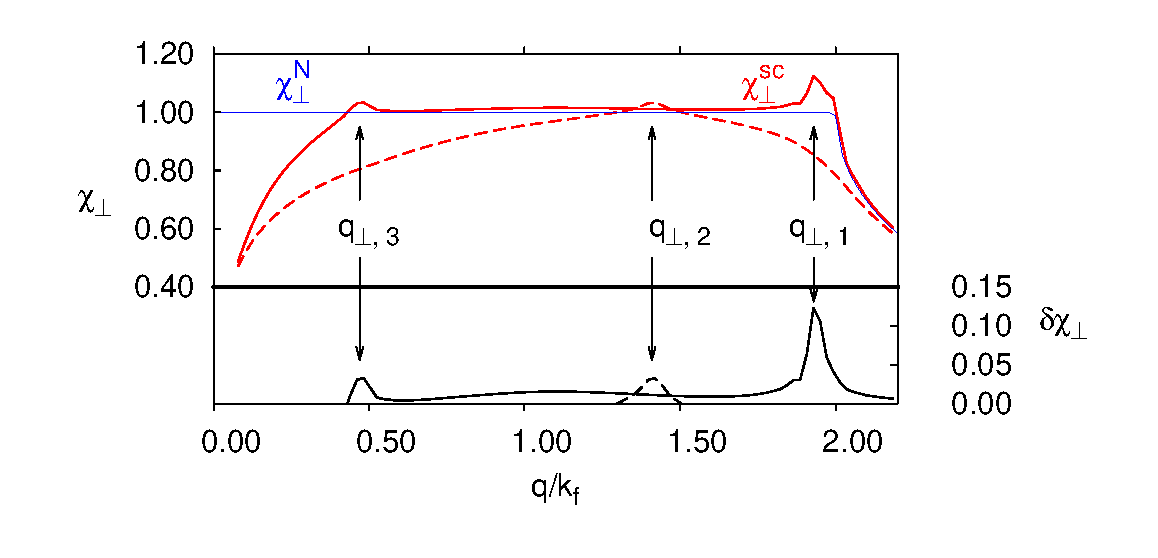
\includegraphics[scale = 0.5]{./figures/enhanced_chi_xx.eps}
                \caption{\begin{flushleft} The upper pane is the transverse susceptibility in the superconducting state (red) as a function of q shows enhancement over the normal state (blue) at the expected wave vectors ($\vq_{\perp1}$, $\vq_{\perp 2}$ and $\vq_{\perp 3}$). The solid red line is along the $\vq_{\perp 1}/\vq_{\perp 3}$ direction, while the dotted line is for q's taken along the direction of $\vq_{\perp 2}$. The lower pane shows $\delta\chi_\perp = \chi_\perp^{sc} - \chi_\perp^{N}$.  $\Delta_0 = 0.1\epsilon_f$, $\mu_B H = 0.5\Delta_0$, $T=0$ \end{flushleft} \label{fig:xx_enh}}

 \end{figure}
 %%%%%%%%%%%%%%%%%%%%%%%%%%%%%%%%%%%%%%%%%%%%%%%%%%%%%%%%%%%%%%%%%%%%%%%%%%%%%%%%%
  
 %%%%%%%%%%%%%%%%%%%%%%%%%%%%%%%%%%%%%%%%%%%%%%%%%%%%%%%%%%%%%%%%%%%%%%%%%%%%%%%%%
 \begin{figure}
        \centering
                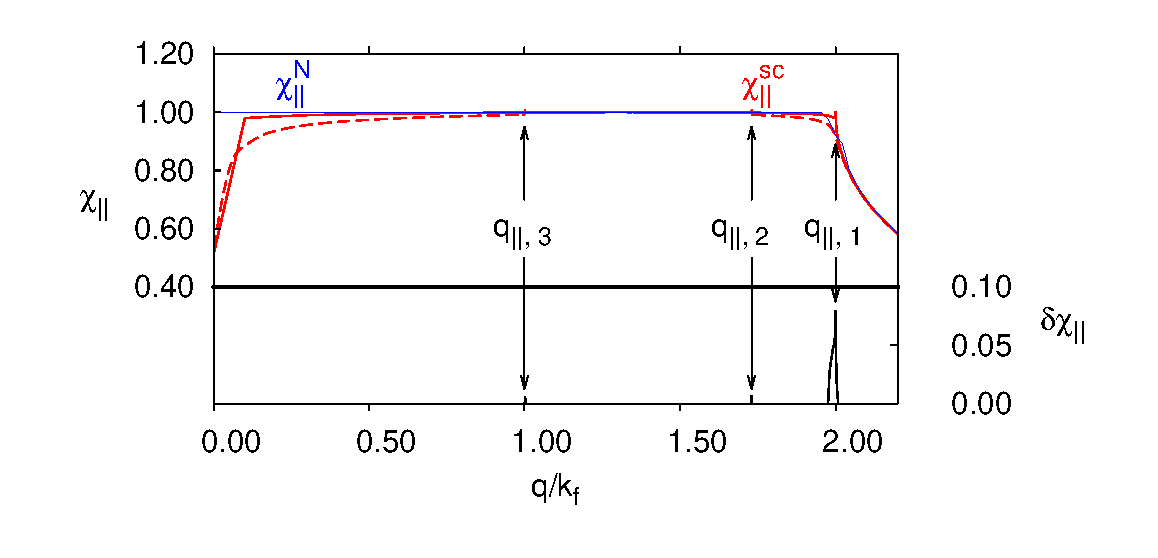
\includegraphics[scale = 0.5]{./figures/enhanced_chi_zz.eps}
                \caption{\begin{flushleft} The upper pane is the longitudinal susceptibility in the superconducting state (red) as a function of q shows enhancement over the normal state (blue) at the expected wave vectors ($\vq_{\parallel 1}$, $\vq_{\parallel 2}$ and $\vq_{\parallel 3}$). The solid red line is along the $\vp_{\parallel,1}$ direction, while the dotted line is for q's taken along the direction of $\vq_{\parallel 2}/\vq_{\parallel 3}$. The lower pane shows $\delta\chi_\parallel = \chi_\parallel^{sc} - \chi_\parallel^{N}$.  $\Delta_0 = 0.01\epsilon_f$, $\mu_B H = 0.5\Delta_0$, $T=0$ \end{flushleft} \label{fig:zz_enh}}

 \end{figure}
 %%%%%%%%%%%%%%%%%%%%%%%%%%%%%%%%%%%%%%%%%%%%%%%%%%%%%%%%%%%%%%%%%%%%%%%%%%%%%%%%%
At zero temperature we find that all the wave vectors described above do lead to some amount of enhancement of the magnetic susceptibility in the superconducting state (figs \ref{fig:xx_enh}, \ref{fig:zz_enh}). However, the enhancement is negligable for $\vq_{\parallel 2}$ and $\vq_{\parallel 3}$ for reasons we do not understand. 

 %%%%%%%%%%%%%%%%%%%%%%%%%%%%%%%%%%%%%%%%%%%%%%%%%%%%%%%%%%%%%%%%%%%%%%%%%%%%%%%%%
 \begin{figure}
        \centering
                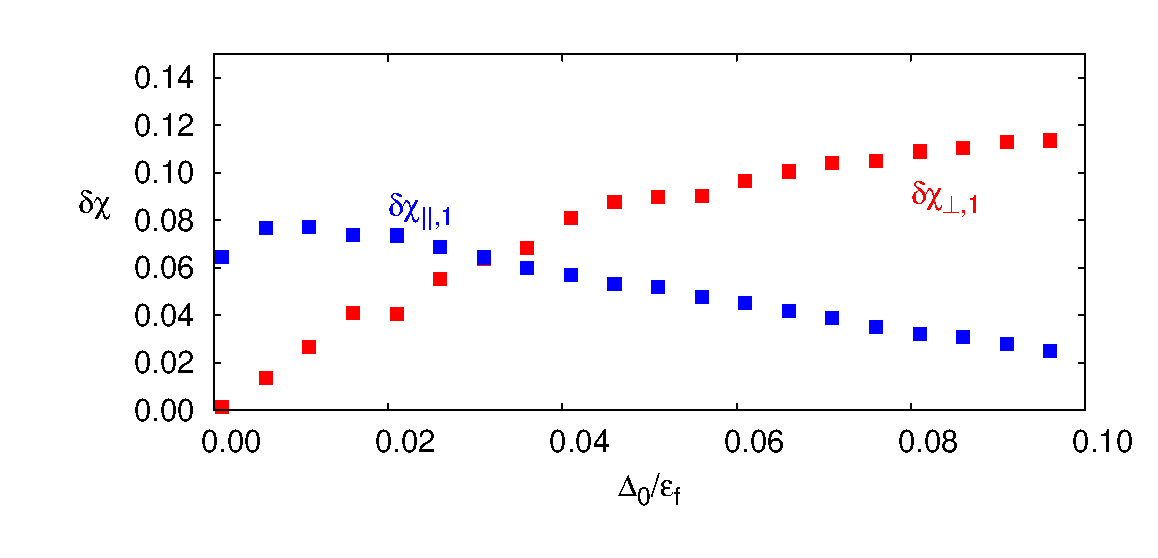
\includegraphics[width=0.45\textwidth]{./figures/delta_dep_q1.eps}
                \caption{\begin{flushleft} The enhancement of both components as a function of $\Delta_0/\epsilon_f$ at $\vq_{\parallel,1}$ and $\vq_{\perp,1}$ respectively.\end{flushleft}\label{fig:deltaDep}}

 \end{figure}
 %%%%%%%%%%%%%%%%%%%%%%%%%%%%%%%%%%%%%%%%%%%%%%%%%%%%%%%%%%%%%%%%%%%%%%%%%%%%%%%%%
 
In figures \ref{fig:xx_enh} and \ref{fig:zz_enh} we have chosen to use $\Delta_0 = 0.1\epsilon_f$ and $\Delta_0 = 0.01\epsilon_f$ respectfully. The reason for this can be seen in figure \ref{fig:deltaDep} which clearly shows that the two components respond in oppsition to an increasing order parameter, and that $\delta\chi_\parallel$ reaches a maximum somewhere near $\Delta_0 = 0.01\epsilon_f$.  

To better understand this enhancement, and it's possible application to the material CeCoIn$_5$ we also investigated the temperature and field dependence of the enhancement (figs \ref{fig:xx_cont}, \ref{fig:zz_cont}). The contours seen here retain their general shape regaurdless of the value of $\Delta_0/\epsilon_f$ and show qualitative agreement with the Q-phase boundary seen in CeCoIn$_5$ which is indicated by the bold red line.

Yet another point of interest is  the behavior of the ideal wave vector $\vq^*$ as a function of applied field and temperature(fig. \ref{fig:qWithT}). To find $\vq^*$ we find the enhancement at various $\vq$'s near the predicted value and pick that which gives a maximum. As
temperature increases the critical wave vector begins to deviate away from the
zero temperature case in such a way that it overlaps the fermi pockets more
($|\bf{q}|$ becomes smaller for both components). 

%The longitudinal wave vector $\vq_{\parallel 2}$deviates most significantly from the predicted
%value in direction, but not magnitude.  In fact, it becomes purely nodal for $T>~0.25T_c$. This deviation seems more drastic than that of the transverse case. We propose
%two possible reasons for this result. Firstly, under an applied field, $\chi^N_{\parallel}$ begins to
%drop off for $|\bf{q}|<2k_f$ (fig. \ref{fig:norm}). Thus, there is a competition between
%this drop off and the enhancement in $\delta \chi$ which may cause the system
%to prefer a $\bf q$ which is more nodal for higher temperatures. Secondly,
%$\bf{q}_{\parallel 2}$ connects the points of zero excitation energy in such a
%way that the pockets are touching, not overlapping slightly as in the
%transverse case (fig. \ref{fig:integrand}). For finite temperature the edges of these pockets
%get smeared out, thus affecting the longitudinal more dramatically and causing the system to find a more different maximum.


 %%%%%%%%%%%%%%%%%%%%%%%%%%%%%%%%%%%%%%%%%%%%%%%%%%%%%%%%%%%%%%%%%%%%%%%%%%%%%%%%%
 \begin{figure}
        \centering
                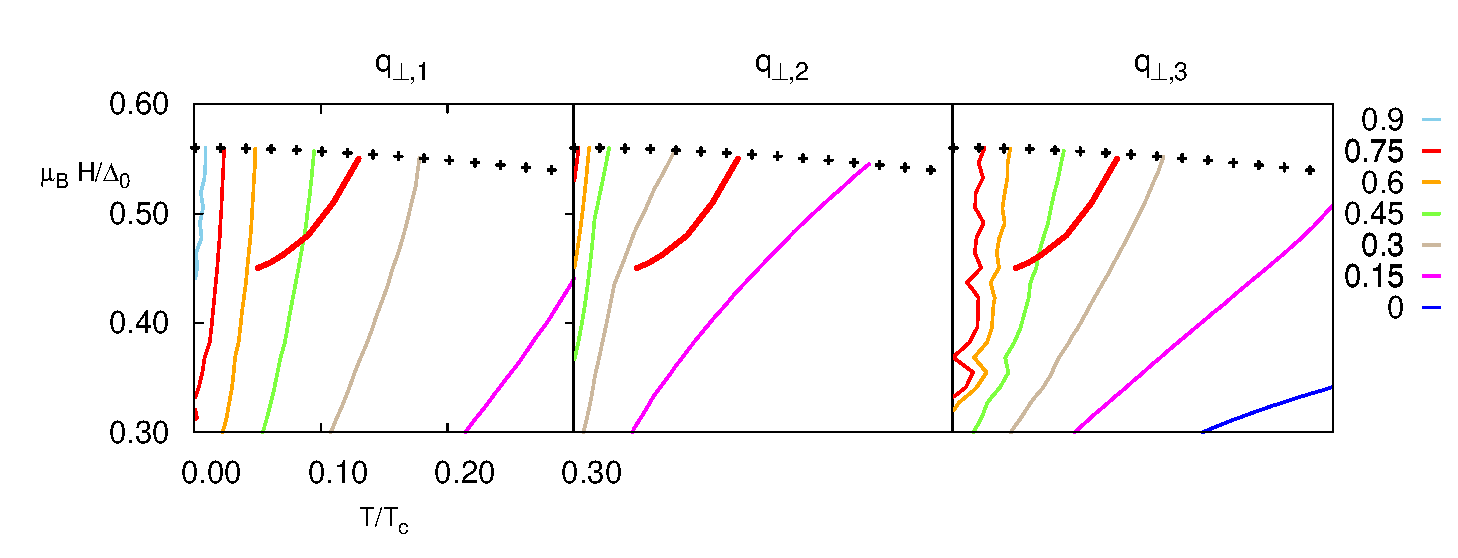
\includegraphics[width=0.5\textwidth]{./figures/xx_all_enhanced_q.eps}
                \caption{\begin{flushleft} Percent increase of $\chi_{\perp}$ for the critical wave vectors in figure \ref{fig:qq}. The black bold dotted line is the first order phase transition for a Pauli limited d-wave superconductor, and the bold red line is a qualitative sketch of the Q-phase boundary of CeCoIn$_5$.  $\Delta_0 = 0.005\epsilon_f$\end{flushleft} \label{fig:xx_cont}}

 \end{figure}
 %%%%%%%%%%%%%%%%%%%%%%%%%%%%%%%%%%%%%%%%%%%%%%%%%%%%%%%%%%%%%%%%%%%%%%%%%%%%%%%%%
 %%%%%%%%%%%%%%%%%%%%%%%%%%%%%%%%%%%%%%%%%%%%%%%%%%%%%%%%%%%%%%%%%%%%%%
 \begin{figure}
        \centering
                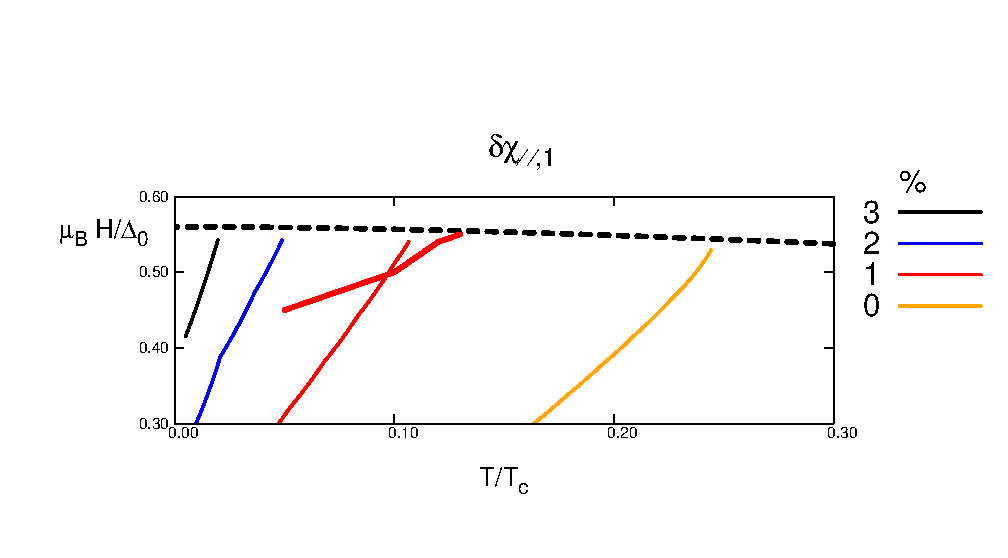
\includegraphics[width = 0.5\textwidth]{./figures/zz_contours_1.eps}
                \caption{\begin{flushleft}Percent increase of $\chi_{\parallel}$ for the critical wave vector in figure \ref{fig:qq} $\vq_{\parallel 1}$. The black bold dotted line is the 
                first order phase transition for a Pauli limited d-wave superconductor, and the bold red line is a qualitative sketch of the Q-phase boundary of
                CeCoIn $_5$.  $\Delta_0 = 0.01\epsilon_f$\end{flushleft} \label{fig:zz_cont}}
 \end{figure}
 %%%%%%%%%%%%%%%%%%%%%%%%%%%%%%%%%%%%%%%%%%%%%%%%%%%%%%%%%%%%%%%%%%%%%%%%

%%%%%%%%%%%%%%%%%%%%%%%%%%%%%%%%%%%%%%%%%%%%%%%%%%%%%%%%%%%%%%%%%%%%%%%%%%%%%%%%%
 \begin{figure}
        \centering
                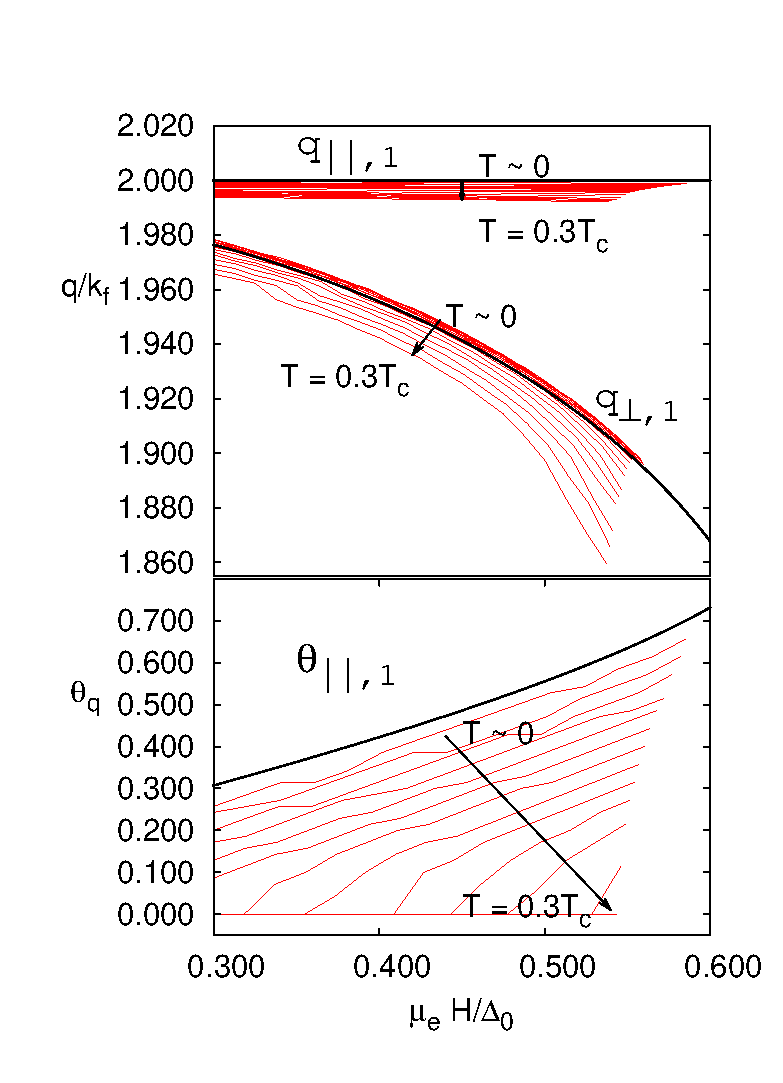
\includegraphics[width=0.45\textwidth]{./figures/max_q_T.eps}
                \caption{\begin{flushleft}The ideal wave vector magnitude for both components depend on temperature and applied field. The black lines are the theoretical curves for $\vq_{\parallel,1}$ and $\vq_{\perp,1}$, and the red lines are found by adaptively finding the maximum in susceptibility. $\Delta_0 = 0.005\epsilon_f$\end{flushleft}\label{fig:qWithT}}

 \end{figure}
 %%%%%%%%%%%%%%%%%%%%%%%%%%%%%%%%%%%%%%%%%%%%%%%%%%%%%%%%%%%%%%%%%%%%%%%%%%%%%%%%%
 
 %~~~~~~~~~~~~~~~~~~~~~~~~~~~~~~~~~~~~~
\section{conclusions}
%~~~~~~~~~~~~~~~~~~~~~~~~~~~~~~~~~~~~~
%
We find that for certain ordering wave vectors (fig \ref{fig:qq}), the superconducting magnetic
susceptibility becomes enhanced over the normal state. At zero temperature,
these ideal wave vectors connect points on the zero field fermi surface
corresponding to zero qusiparticle excitation energy $\epsilon_{\vk,s}$ which
can only occur for order parameters which become sufficiently small.

Due to the terms in equation \ref{eq:xi} which drive this enhancement we can also
conclude that the enhancement in $\chi^{sc}_{\perp}$ can only occur for order
parameters which are explicitely nodal (ie change sign) becuase the ideal $\vq$'s connect
points of zero excitation energy and opposite signs of the order parameter.
This contrasts with the longitudinal component which prefers wave vectors which
connect regions of the same sign of the order parameter. Thus, the longitudinal
componenet may become enhanced for strongly anisotropic superconductors if the
order parameter becomes sufficiently small.

We believe that the enhancement of $\chi$ may be enough to establish magnetic
order inside the superconducting state. In the case of CeCoIn$_5$ it may also
explain the collapse of AMF with superconductivity at H$_{c2}$. 

This conclusion follows from the equation for total susceptibility in terms of the first order
expansion and the magnetic interaction. 

\begin{align}
\chi^{total}_{\alpha\beta}=\frac{\chi_{\alpha\beta}}{1-J_{\alpha\beta} \chi_{\alpha\beta}}
\end{align}

If a normal state material were to have a susceptibility and magnetic interaction, $J_{\alpha\beta}$, such that
$1-J_{\alpha\beta} \chi_{\alpha\beta}<<1$, then a small enhancement of
$\chi_{\alpha\beta}$ could be sufficent to induce magnetic order. 

In the case of itinerant electrons, this order would be in the form of a spin density wave
(SDW). The origins of the magnetic interaction $J_{\alpha\beta}$ are not
discussed here, but may be from coupling to the localized magnetic moments of
the Ce atoms, (RKKY interaction \cite{x}) or by some other mechanism.

We also note the field dependence of the various critical $\vq$'s identified in this paper (fig \ref{fig:qqTheory}), which has not been addressed in many of the other theories which try to explain the origins of the Q-phase of CeCoIn$_5$. Experimental evidence points to a near constant or possibly increasing $|\vq|$ which is consistent with $\vq_{\perp,2}$, $\vq_{\perp,3}$, $\vq_{\parallel,1}$ or $\vq_{\parallel,2}$. \cite{sc_sdw_anton,mag_afm_fflo_sigrist,fflo_pen_depth,sc_afm_kato,sc_afm_ikeda,sdw_vortex, cecoin5_Kenzelmann2}

With these considerations in mind along with the contours in \ref{fig:xx_cont} we feel that $\vq_{\perp,2}$ is the best candidate for the Q-phase of CeCoIn$_5$.



%One key feature of the critical values at which $\chi^{sc}$ is maximized is that $q^*$ is a decreasing function of applied field. FFLO state calculations also have this feature. However, experimental results in CeCoIn$_5$ show a small increase in $q^*$ with increasing field.\cite{cecoin5_Kenzelmann2} This fact is often ignored in many theories, but may provide a deeper insight into the phenomenon which is not yet understood.\cite{spin_sus_dyn,sdw_vortex,sc_afm_ikeda,sc_afm_kato,mag_afm_fflo_sigrist,sc_sdw_anton}

 %~~~~~~~~~~~~~~~~~~~~~~~~~~~~~~~~~~~~~~~~~~~~~~~~~~~~~~~~~~~~~~~~~~~~~~~~~~~~~~~
  %~~~~~~~~~~~~~~~~~~~~~~~~~~~~~~~~~~~~~~~~~~~~~~~~~~~~~~~~~~~~~~~~~~~~~~~~~~~~~~~
   %~~~~~~~~~~~~~~~~~~~~~~~~~~~~~~~~~~~~~~~~~~~~~~~~~~~~~~~~~~~~~~~~~~~~~~~~~~~~~~~
    %~~~~~~~~~~~~~~~~~~~~~~~~~~~~~~~~~~~~~~~~~~~~~~~~~~~~~~~~~~~~~~~~~~~~~~~~~~~~~~~
     %~~~~~~~~~~~~~~~~~~~~~~~~~~~~~~~~~~~~~~~~~~~~~~~~~~~~~~~~~~~~~~~~~~~~~~~~~~~~~~~
      %~~~~~~~~~~~~~~~~~~~~~~~~~~~~~~~~~~~~~~~~~~~~~~~~~~~~~~~~~~~~~~~~~~~~~~~~~~~~~~~
\appendix
\begin{widetext}


 %~~~~~~~~~~~~~~~~~~~~~~~~~~~~~~~~~~~~~~~~~~~~~~~~~~~~~~~~~~~~~~~~~~~~~~~~~~~~~~~
\section{\label{sec:appA} Susceptibility in magnetic field} 
 %~~~~~~~~~~~~~~~~~~~~~~~~~~~~~~~~~~~~~~~~~~~~~~~~~~~~~~~~~~~~~~~~~~~~~~~~~~~~~~~

The presence of a magnetic field introduces a potential for particles with spin $V=-\vec{m}\cdot\vec{H}$. The magnetization due to this potential is given by $M_\alpha(t)=-i\int\limits_{-\infty}^t <[m_\alpha(t),V(t')]>dt'$. For the case of uniform space and time, tthe magnetic susceptibility is $\chi_{\alpha,\beta}(\vx,t)=i<[m_\alpha(0,0),m_\beta(\vx,t)]\Theta(t)>dt'$. The magnetic moment is given by $m_\alpha(\vx,t)=\mu_e\sum\limits_{\mu,\mu'} \sigma^{\alpha}_{\mu,\mu'}\psi^\dagger_\mu(\vx,t) \psi_{\mu'}(\vx,t)$ ~\cite{mahan}. Now we can proceed to calculate the susceptibitily.
\begin{align*}
\chi_{\alpha\beta}(\vx, \omega)=-i \mu_B^2\sum\limits_{\mu\mu'\nu\nu'}\int\limits_0^{\infty}dt' \; \sigma^\alpha_{\nu\nu'}\sigma^\beta_{\mu\mu'}e^{i\omega t'} \; 
\langle [\psi^\dagger_\mu(\vx ,t') \psi_{\mu'}(\vx,t'),  \psi^\dagger_\nu(0,0) \psi_{\nu'}(0,0) ]\rangle
\end{align*}

From now on we will use the $\mu$ and $\mu'$ subscripts to denote the spin for the $(\vx,t')$ coordinates while the $\nu$ and $\nu'$ subscripts denote the spin for the $(0,0)$ coordinates so that $\psi^\dagger_{\mu}=\psi^\dagger_{\mu}(\vx,t')$ and $\psi^\dagger_{\nu}=\psi^\dagger_{\nu}(0,0)$. The correlation function inside the integral evaluates as follows.

\begin{align*}
<[\psi^\dagger_{\mu} \psi_{\mu'},\psi^\dagger_{\nu} \psi_{\nu'}]>=&<\psi^\dagger_{\mu} \psi_{\mu'}\psi^\dagger_{\nu} \psi_{\nu'}>-<\psi^\dagger_{\nu} \psi_{\nu'}\psi^\dagger_{\mu} \psi_{\mu'}> \\
=&-<\psi^\dagger_{\mu}\psi^\dagger_{\nu}><\psi_{\mu'}\psi_{\nu'}>+<\psi^\dagger_{\mu}\psi_{\nu'}><\psi_{\mu'}\psi^\dagger_{\nu}> \\ 
&+<\psi^\dagger_{\nu}\psi^\dagger_{\mu}><\psi_{\nu'}\psi_{\mu'}>-<\psi^\dagger_{\nu}\psi_{\mu'}><\psi_{\nu'}\psi^\dagger_{\mu}> \\
\end{align*}

To evaluate these various correlation functions we use the Bogoliubov representation for the field operators $\psi_\mu = \sum\limits_{\vk}u_\vk \gamma_{\vk \mu} + \sum\limits_{\mu'}(i\sigma_2)_{\mu\mu'} v_\vk^* \gamma^\dag_{-\vk \mu'}=\sum\limits_\vk \Gamma_{\vk,\mu}(x,t)-\Gamma_{\vk,-\mu}^\dagger(x,t)$, where $u_\vk(\vx)$ and $v_\vk(\vx)$ are, in general, complex functions and the $\gamma$'s are new fermionic quasi-particle operators ($\Gamma_{\vk,\mu}(\vx,t)=\gamma_{\vk,\mu}(t)u_\vk(\vx)$, $\Gamma_{\vk,-\mu}^\dagger(\vx,t)=\mu\gamma_{-\vk,-\mu}^\dagger(t)v^*_{\vk}(\vx)$). We find the time dependence of the $\gamma$ operators via the Heisenberg representation, $\frac{d}{dt}\gamma_{\vk\mu}=\frac{i}{\hbar}[H,\gamma_{\mu\vk}]=\frac{-i\epsilon_{\vk\mu}}{\hbar}\gamma_{\vk\mu}$ and $\frac{d}{dt}\gamma^\dagger_{\vk\mu}=\frac{i\epsilon_{\vk\mu}}{\hbar}\gamma^\dagger_{\vk\mu}$.

\begin{equation*}
\gamma_{\vk\mu}(t)=\gamma_{\vk\mu}e^{-i\omega_{\vk\mu}t}\quad\quad \gamma^\dagger_{\vk\mu}(t)=\gamma^\dagger_{\vk\mu}e^{i\omega_{\vk\mu}t}
\end{equation*}

And the correlation relations for the $\gamma$'s are:

\begin{equation*}
<\gamma^\dagger_{\vk\mu}\gamma_{\vp\nu}>=\delta_{\vp\vk}\delta_{\mu\nu}f(\epsilon_{\vk\mu}) \quad\quad <\gamma_{\vk\mu}\gamma_{\vp\nu}>=<\gamma^\dagger_{\vk\mu}\gamma^\dagger_{\vp\nu}>=0
\end{equation*}

Where $f(\epsilon_{\vk\mu})=f_{\vk\mu}=(e^{\beta{\epsilon_{\vk\mu}}}+1)^{-1}$ is the fermi distribution. Using the definition of $\Gamma$ and omitting the time bit, we can deduce the following rules:

\begin{equation*}
<\Gamma^\dagger_{\vk\mu}\Gamma_{\vp\nu}>=\delta_{\vp\vk}\delta_{\mu\nu}f(\epsilon_{\vk\mu})u^*_\vk u_\vp \quad <\Gamma^\dagger_{\vk\mu}\Gamma_{\vp-\nu}>=\beta\delta_{\vp\vk}\delta_{\mu -\nu}f(\epsilon_{\vk\mu})u^*_\vk v_\vp \quad <\Gamma^\dagger_{\vk-\mu}\Gamma_{\vp-\nu}>=\delta_{\vp\vk}\delta_{\mu\nu}f(\epsilon_{\vk\mu})v_\vk v^*_\vp
\end{equation*}

Going back to the sum of wick contractions, and dropping the quantum number subscript on the $\Gamma$'s:

\begin{align*}
<[\psi^\dagger_{\mu} \psi_{\mu'},\psi^\dagger_{\nu} \psi_{\nu'}]>=&-(<\Gamma^\dagger_{\mu}\Gamma_{-\nu}>+<\Gamma_{-\mu}\Gamma^\dagger_{\nu}>)(<\Gamma_{\mu'}\Gamma^\dagger_{-\nu'}>+<\Gamma^\dagger_{-\mu'}\Gamma_{\nu'}>) \\ &+(<\Gamma^\dagger_{\mu}\Gamma_{\nu'}>+<\Gamma_{-\mu}\Gamma^\dagger_{-\nu'}>)(<\Gamma_{\mu'}\Gamma^\dagger_{\nu}>+<\Gamma^\dagger_{-\mu'}\Gamma_{-\nu}>) \\ 
&+(<\Gamma^\dagger_{\nu}\Gamma_{-\mu}>+<\Gamma_{-\nu}\Gamma^\dagger_{\mu}>)(<\Gamma_{\nu'}\Gamma^\dagger_{-\mu'}>+<\Gamma^\dagger_{-\nu'}\Gamma_{\mu'}>) \\
&-(<\Gamma^\dagger_{\nu}\Gamma_{\mu'}>+<\Gamma_{-\nu}\Gamma^\dagger_{-\mu'}>)(<\Gamma_{\nu'}\Gamma^\dagger_{\mu}>+<\Gamma^\dagger_{-\nu'}\Gamma_{-\mu}>)
\end{align*}

\begin{align*}
=\sum\limits_{\vk\vp}\delta_{\mu\nu'}\delta_{\mu'\nu}&\bigg[[T^*_{\vk\mu}f_{\vk\mu}u^*_\vk(\vx)u_\vk+T_{-\vk-\mu}(1-f_{-\vk-\mu})v_{-\vk}(\vx)v^*_{-\vk}][T_{\vp\mu'}(1-f_{\vp\mu'})u_\vp(\vx)u^*_\vp+T^*_{-\vp-\mu'}f_{-\vp-\mu'}v^*_{-\vp}(\vx)v_{-\vp}] \\ 
&-[T_{\vp\mu'}f_{\vp\mu'}u^*_\vp u_\vp(\vx)+T^*_{-\vp-\mu'}(1-f_{-\vp-\mu'})v_{-\vp}v^*_{-\vp}(\vx)] [T^*_{k\mu}(1-f_{k\mu})u_\vk u^*_\vk(\vx)+T_{-\vk-\mu}f_{-\vk-\mu}v^*_{-\vk}v_{-\vk}(\vx)]\bigg] 
\\ 
+\mu\mu'\delta_{\mu-\nu}\delta_{\mu'-\nu'}&\bigg[-[T_{-\vk-\mu}(1-f_{-\vk-\mu})u^*_{-\vk}v_{-\vk}(\vx)-T^*_{\vk\mu}f_{\vk\mu}v_\vk u^*_\vk (\vx)][-T_{\vp\mu'}(1-f_{\vp\mu'})v^*_\vp u_\vp(\vx)+T^*_{-\vp-\mu'}f_{-\vp-\mu'}u_{-\vp}v^*_{-\vp}(\vx)] \\ 
&+ [T_{-\vk-\mu}f_{-\vk-\mu}v_{-\vk}(\vx)u^*_{-\vk}-T^*_{\vk\mu}(1-f_{\vk\mu})u^*_\vk (\vx)v_\vk][T^*_{-\vp-\mu'}(1-f_{-\vp-\mu'})v^*_{-\vp}(\vx)u_{-\vp}-T_{\vp\mu'}f_{\vp\mu'}u_p(\vx)v^*_p]\bigg]
\end{align*}

Where $T_{k\mu}=e^{-i\omega_{\vk\mu}\tau}$ which carries the time dependence from the $\gamma$ operators. 

%\begin{align*}
%=\sum\limits_{kp}\delta_{st'}\delta_{s't}\bigg[(f_{ks}-f_{ps'})u^*_pu_p(r)u_ku^*_k(r) e^{i(\omega_{ks}-\omega_{ps'})\tau}
%+(1-f_{ps'}-f_{-k-s})u^*_pu_p(r)v^*_{-k}v_{-k}(r) e^{-i(\omega_{-k-s}+\omega_{ps'})\tau}\\
%+(-1+f_{-p-s'}+f_{ks})v_{-p}v^*_{-p}(r)u_ku^*_k(r) e^{i(\omega_{-p-s'}+\omega_{ks})\tau}
%+(f_{-p-s'}-f_{-k-s})v_{-p}v^*_{-p}(r)v^*_{-k}v_{-k}(r) e^{i(\omega_{-p-s'}-\omega_{-k-s})\tau}\bigg] 
%\\
%+ss'\delta_{s-t}\delta_{s'-t'}\bigg[(1-f_{-k-s}-f_{ps'})u^*_{-k}v_{-k}(r)v^*_pu_p(r) e^{-i(\omega_{ps'} + \omega_{-k-s})\tau}
%+(f_{-k-s}-f_{-p-s'})u^*_{-k}v_{-k}(r)v^*_{-p}(r)u_{-p}e^{i(\omega_{-p-s'}-\omega_{-k-s})\tau} \\
%-(f_{ps'}-f_{ks})u^*_k(r)v_kv^*_pu_p(r) e^{i(\omega_{ks}-\omega_{ps'})\tau}
%-(1-f_{ks}-f_{-p-s'})u^*_k(r)v_kv^*_{-p}(r)u_{-p} e^{i(\omega_{ks}+\omega_{-p-s'})\tau}\bigg]
%\end{align*}

Now we transform to frequency space by multiplying the entire integral by $e^{- \delta t'}$, and preform the integration in $t'$.
\begin{align*}
\chi_{\alpha\beta}(\omega,q) = -\mu_B^2 \sum\limits_{\vk\vp\mu\mu'} \sigma^\beta_{\mu\mu'}\sigma^\alpha_{\mu'\mu}\bigg[\frac{(f_{\vk\mu}-f_{\vp\mu'})u^*_\vp u_\vp(\vx)u_\vk u^*_\vk(\vx)}{\omega+\omega_{\vk\mu}-\omega_{\vp\mu'}+i\delta}
+\frac{(1-f_{\vp\mu'}-f_{-\vk-\mu})u^*_\vp u_\vp(\vx)v^*_{-\vk}v_{-\vk}(\vx)}{\omega-\omega_{-\vk-\mu}-\omega_{\vp\mu'}+i\delta}\\
+\frac{(-1+f_{-\vp-\mu'}+f_{\vk\mu})v_{-\vp}v^*_{-\vp}(\vx)u_\vk u^*_\vk(\vx)}{\omega+\omega_{-\vp-\mu'}+\omega_{\vk\mu}+i\delta}
+\frac{(f_{-\vp-\mu'}-f_{-\vk-\mu})v_{-\vp}v^*_{-\vp}(\vx)v^*_{-\vk}v_{-\vk}(\vx)}{\omega+\omega_{-\vp-\mu'}-\omega_{-\vk-\mu}+i\delta}\bigg] 
\\
+\mu\mu' \sigma^\beta_{\mu\mu'}\sigma^\alpha_{-\mu-\mu'}\bigg[\frac{(1-f_{-\vk-\mu}-f_{\vp\mu'})u^*_{-\vk}v_{-\vk}(\vx)v^*_\vp u_\vp(\vx)}{\omega-\omega_{\vp\mu'} - \omega_{-\vk-\mu}+i\delta}
+\frac{(f_{-\vk-\mu}-f_{-\vp-\mu'})u^*_{-\vk}v_{-\vk}(\vx)v^*_{-\vp}(\vx)u_{-\vp}}{\omega+\omega_{-\vp-\mu'}-\omega_{-\vk-\mu}+i\delta} \\
-\frac{(f_{\vp\mu'}-f_{\vk\mu})u^*_\vk(\vx)v_\vk v^*_\vp u_\vp(\vx)}{\omega+\omega_{\vk\mu}-\omega_{\vp\mu'}+i\delta}
-\frac{(1-f_{\vk\mu}-f_{-\vp-\mu'})u^*_\vk(\vx)v_\vk v^*_{-\vp}(\vx)u_{-\vp}}{\omega+\omega_{\vk\mu}+\omega_{-\vp-\mu'}+i\delta}\bigg]
\end{align*}

Now we Fourier transform to momentum space by using the equations for u's and v's from the Bogolioubov equations $u_\vk(\vx)=u_\vk e^{i\vk\cdot\vx}$ and $v_\vk(\vx)=v_\vk e^{i\vk\cdot\vx}$, $\bigg(u_\vk = \sqrt{\frac{1}{2}(1+\frac{\xi_\vk}{\epsilon_\vk})},\quad v_\vk = sgn(\Delta_\vk)\sqrt{\frac{1}{2}(1-\frac{\xi_\vk}{\epsilon_\vk})}\bigg)$

\begin{align*}
\chi_{\alpha\beta}(\omega,\vq) = -\mu_B^2 \sum\limits_{\vk,\mu,\mu'} \sigma^\beta_{\mu\mu'}\sigma^\alpha_{\mu'\mu}\bigg[\frac{(f_{\vk\mu}-f_{\vk+\vq\mu'})u_{\vk+\vq}^2u_\vk^2} {\omega+ \omega_{\vk\mu}-\omega_{\vk+\vq\mu'}+i\delta}
+\frac{(1-f_{\vk+\vq\mu'}-f_{\vk-\mu})u_{\vk+\vq}^2v_\vk^2} {\omega-\omega_{\vk-\mu}-\omega_{\vk+\vq\mu'}+i\delta}\\
+\frac{(-1+f_{\vk+\vq-\mu'}+f_{\vk\mu})v_{\vk+\vq}^2u_\vk^2} {\omega+\omega_{\vk+\vq-\mu'}+\omega_{\vk\mu}+i\delta}
+\frac{(f_{\vk+\vq-\mu'}-f_{\vk-\mu})v_{\vk+\vq}^2v_\vk^2} {\omega+\omega_{\vk+\vq-\mu'}-\omega_{\vk-\mu}+i\delta}\bigg] 
\\
+\mu\mu' \sigma^\beta_{\mu\mu'}\sigma^\alpha_{-\mu-\mu'}\bigg[\frac{(1-f_{\vk-\mu}-f_{\vk+\vq\mu'})u_\vk v_\vk v_{\vk+\vq}u_{\vk+\vq}} {\omega-\omega_{\vk+\vq\mu'} - \omega_{\vk-\mu}+i\delta}
+\frac{(f_{\vk-\mu}-f_{\vk+\vq-\mu'})u_\vk v_\vk v_{\vk+\vq}u_{\vk+\vq}} {\omega+\omega_{\vk+\vq-\mu'}-\omega_{\vk-\mu}+i\delta} \\
-\frac{(f_{\vk+\vq\mu'}-f_{\vk\mu})u_\vk v_\vk v_{\vk+\vq}u_{\vk+\vq}} {\omega+\omega_{\vk\mu}-\omega_{\vk+\vq\mu'}+i\delta}
-\frac{(1-f_{\vk\mu}-f_{\vk+\vq-\mu'})u_\vk v_\vk v_{\vk+\vq}u_{\vk+\vq}} {\omega+\omega_{\vk\mu}+\omega_{\vk+\vq-\mu'}+i\delta}\bigg]
\end{align*}

The susceptibility is then:

\begin{align*}
\chi_{\alpha\beta}(\omega,q) =- \mu_B^2 \sum\limits_{\vk,\mu,\mu'} \sigma^\beta_{\mu\mu'}\sigma^\alpha_{\mu'\mu} \bigg[\frac{(f^+_{\vk\mu}-f^+_{\vk+\vq\mu'})u_{\vk+\vq}^2u_\vk^2} {\omega+\omega^+_{\vk\mu}- \omega^+_{\vk+\vq\mu'}+i\delta}
+\frac{(f^-_{\vk\mu}-f^+_{\vk+\vq\mu'})u_{\vk+\vq}^2v_\vk^2} {\omega+\omega^-_{\vk\mu}-\omega^+_{\vk+\vq\mu'}+i\delta}\\
+\frac{(f^+_{\vk\mu}-f^-_{\vk+\vq\mu'})v_{\vk+\vq}^2u_\vk^2} {\omega+\omega^+_{\vk\mu}-\omega^-_{\vk+\vq\mu'}+i\delta}
+\frac{(f^-_{\vk\mu}-f^-_{\vk+\vq\mu'})v_{\vk+\vq}^2v_\vk^2} {\omega+\omega^-_{\vk\mu}-\omega^-_{\vk+\vq\mu'}+i\delta}\bigg] 
\\
+\mu\mu' \sigma^\beta_{\mu\mu'}\sigma^\alpha_{-\mu-\mu'}\bigg[\frac{(f^-_{\vk\mu}-f^+_{\vk+\vq\mu'})u_\vk v_\vk v_{\vk+\vq}u_{\vk+\vq}} {\omega+ \omega^-_{\vk\mu}-\omega^+_{\vk+\vq\mu'} +i\delta}
-\frac{(f^-_{\vk\mu}-f^-_{\vk+\vq\mu'})u_\vk v_\vk v_{\vk+\vq}u_{\vk+\vq}} {\omega+\omega^-_{\vk\mu}-\omega^-_{\vk+\vq\mu'}+i\delta} \\
-\frac{(f^+_{\vk\mu}-f^+_{\vk+\vq\mu'})u_\vk v_\vk v_{\vk+\vq}u_{\vk+\vq}} {\omega+\omega^+_{\vk\mu}-\omega^+_{\vk+\vq\mu'}+i\delta}
+\frac{(f^+_{\vk\mu}-f^-_{\vk+\vq\mu'})u_\vk v_\vk v_{\vk+\vq}u_{\vk+\vq}} {\omega+\omega^+_{\vk\mu}-\omega^-_{\vk+\vq\mu'}+i\delta}\bigg]
\end{align*}

Where we have defined the following:
\begin{align*}
\delta \rightarrow 0^+ \\
\omega^+_{\vk\mu} = \omega_{\vk\mu} \\
\omega^-_{\vk\mu} = -\omega_{\vk-\mu} \\
f^+_{\vk\mu} = f(\epsilon_{\vk\mu}) \\
f^-_{\vk\mu} = f(-\epsilon_{\vk-\mu})
\end{align*}

%~~~~~~~~~~~~~~~~~~~~~~~~~~~~~~~~~~~~~~~~~~~~~~~~~~~~~~~~~~~~~~~~~~~~~~~~~~~~~~~
\section{\label{sec:appB} Normal state susceptibility} 
%~~~~~~~~~~~~~~~~~~~~~~~~~~~~~~~~~~~~~~~~~~~~~~~~~~~~~~~~~~~~~~~~~~~~~~~~~~~~~~~
%
To find the normal state susceptibility at zero temperature we first orient our coordinates such that ${\bf q}=q\hat{x}$, and change from ${\bf k}$ and ${\bf k+q}$ to ${\bf k-q}/2$ and ${\bf k+q}/2$. Converting the sums to integrals, and using symmetry about the x and y axes, we have:
 
 \begin{align*}
 \chi_\parallel=-8\mu_B^2\sum\limits_\mu \int\limits_0^{\pi/2} d\phi \int k dk  \frac{ f(\epsilon_{{\bf k-q}/2,\mu})-f(\epsilon_{{\bf k+q}/2,\mu})}{ -2kq\cos\phi} \\
  \chi_\perp=-8\mu_B^2\sum\limits_{\mu} \int\limits_0^{\pi/2} d\phi \int k dk  \frac{ f(\epsilon_{{\bf k-q}/2,\mu})-f(\epsilon_{{\bf k+q}/2,-\mu})}{ -2kq\cos\phi+2\mu \mu_B H}
 \end{align*}
 Where we have also normalized the 2D area of integration $A/(2\pi \hbar)^2=1$
 %~~~~~~~~~~~~~~~~~~~~~~~~~~~~~~~~~~~~~~~~~~~~~~~~~~~~~~~~~~~~~~~~~~~~~~~~~~~~~~~
 \section*{Longitudinal}
 %~~~~~~~~~~~~~~~~~~~~~~~~~~~~~~~~~~~~~~~~~~~~~~~~~~~~~~~~~~~~~~~~~~~~~~~~~~~~~~~
 To determine the limits of integration on k, we need to solve the dispersion relation for k when $\epsilon_{{\bf k\pm q}/2,s}=\epsilon_f$, the fermi energy. If we normalize the equation by multiplying and dividing it by $k_f^2$, the resulting limits of integration are:
 
 \begin{align*}
k'=\mp \frac{q'\cos\phi}{2} \pm\sqrt{1-sH'-(q'/2)^2\sin^2\phi} = K_{\pm\pm s} \\
\sin{\phi_s}=\frac{2}{q'}\sqrt{1-sH'} 
 \end{align*}
 
 Where $k'=k/k_f$, $q'=q/k_f$ and $H'=\mu_B H/k_f^2$. For the longitudinal component we must consider three regions of q:% {\bf A}) $q\in[0,2\sqrt{1-H'}]$, {\bf B}) $q\in[2\sqrt{1-H'},2\sqrt{1+H'}]$, {\bf C}) $q\in[2\sqrt{1+H'},\infty]$ :
 
 \framebox{{\bf A}) $q'\in[0,2\sqrt{1-H'}]$}
 \begin{align*}
\chi_\parallel&=8\mu_B^2\sum\limits_s \int\limits_0^{\pi/2} d\phi \int\limits_0^{K_{++s}}dk'  \frac{ 1}{ 2q'\cos\phi}-\int\limits_0^{K_{-+s}} dk'  \frac{ 1}{ 2q'\cos\phi} =4\mu_B^2\pi
 \end{align*}
 
 \framebox{{\bf B}) $q'\in[2\sqrt{1-H'},2\sqrt{1+H'}]$}
 \begin{align*}
\chi_\parallel&=2\mu_B^2\pi +8\mu_B^2\int\limits_0^{\phi_1} d\phi \int\limits_{KK_{+-1}}^{K_{++1}}dk'  \frac{ 1}{ 2q'\cos\phi} \\
&=2\mu_B^2\pi +\frac{8\mu_B^2}{q'}\int\limits_0^{\phi_1} d\phi  \frac{ \sqrt{1-H'-(q'/2)^2\sin^2\phi}}{ \cos\phi} \\
&=2\mu_B^2\pi +\frac{8\mu_B^2}{q'}\int\limits_0^{\sin\phi_1} dx  \frac{ \sqrt{1-H'-(q'/2)^2 x^2}}{ 1-x^2}  \\
\chi_\parallel&=4\mu_B^2\pi\bigg[1 - \frac{1}{2}\sqrt{1-(1-H')(2/q')^2}\bigg]  \\
 \end{align*}
 
 
  \framebox{{\bf C}) $q'\in[2\sqrt{1+H'},\infty]$}
   \begin{align*}
\chi_\parallel&=8\mu_B^2\int\limits_0^{\phi_{-1}} d\phi \int\limits_{K_{+-(-1)}}^{K_{++(-1)}}dk'  \frac{ 1}{ 2q'\cos\phi}  +8\mu_B^2\int\limits_0^{\phi_1} d\phi \int\limits_{KK_{+-1}}^{K_{++1}}dk'  \frac{ 1}{ 2q'\cos\phi} \\
\chi_\parallel&=4\mu_B^2\pi\bigg[1 - \frac{1}{2}\sqrt{1-(1+H')(2/q'^2)} -\frac{1}{2}\sqrt{1-(1-H')(2/q')^2}  \bigg]
 \end{align*}
  
  %~~~~~~~~~~~~~~~~~~~~~~~~~~~~~~~~~~~~~~~~~~~~~~~~~~~~~~~~~~~~~~~~~~~~~~~~~~~~~~~
  \section*{Transverse}
  %~~~~~~~~~~~~~~~~~~~~~~~~~~~~~~~~~~~~~~~~~~~~~~~~~~~~~~~~~~~~~~~~~~~~~~~~~~~~~~~
  Now we continue with the perpendicular component. To do this we move the origin such that at $k_x$=0 the s=1 and s=-1 surfaces intersect. The equation for this transformation is $k'_x \rightarrow k'_x-q'/2+sH'/q'$, and the limits of integration are:
 \begin{align*}
k=\pm(q'/2-sH'/q')\cos\phi\pm\sqrt{1-sH'-(q'/2-sH'/q')^2\sin^2\phi} = K_{\pm\pm s} \\ 
\sin{\phi_s}=\frac{2q'\sqrt{1-sH'} }{q'^2-2sH'}
 \end{align*}
 For this integration there are two regions:
 
 \framebox{{\bf A}) $q'\in[0,\sqrt{1+H'}+\sqrt{1-H'}]$}
 \begin{align*}
 \chi_\perp&=8\mu_B^2 \int\limits_0^{\pi/2} d\phi \int\limits_0^{K_{++1}}dk'  \frac{ 1}{ 2q'\cos\phi} -\int\limits_0^{K_{-+1}} dk'  \frac{ 1}{ 2q'\cos\phi} +\int\limits_0^{K_{++(-1)}} dk'  \frac{ 1}{ 2q'\cos\phi} -\int\limits_0^{K_{-+(-1)}} dk'  \frac{ 1}{ 2q'\cos\phi} \\
  \chi_\perp&=(8\mu_B^2/q') \int\limits_0^{\pi/2} d\phi (q'/2-H'/q')+(q'/2+H'/q') \\
  \chi_\perp&=4\mu_B^2\pi\\
 \end{align*}
  
 \framebox{{\bf B}) $q'\in[\sqrt{1+H'}+\sqrt{1-H'},\infty]$}
    \begin{align*}
 \chi_\perp&=8\mu_B^2 \int\limits_0^{\phi_1} d\phi \int\limits_{K_{+-1}}^{K_{++1}}dk'  \frac{ 1}{ 2q'\cos\phi}+\int\limits_0^{\phi_{-1}} d\phi \int\limits_{K_{+-(-1)}}^{K_{++(-1)}} dk'  \frac{ 1}{ 2q'\cos\phi}  \\
  \chi_\perp&=(8\mu_B^2/q') \int\limits_0^{\phi_1} d\phi   \frac{ \sqrt{1-H'-(q'/2-H'/q')^2\sin^2\phi}}{ \cos\phi} 
 + \int\limits_0^{\phi_{-1}} d\phi \frac{  \sqrt{1+H'-(q'/2+H'/q')^2\sin^2\phi}}{ \cos\phi}  \\
   \chi_\perp&=(8\mu_B^2/q') \int\limits_0^{\sin\phi_1} dx \frac{ \sqrt{1-H'-(q'/2-H'/q')^2x^2}}{ 1-x^2} 
 +\int\limits_0^{\sin\phi_{-1}} dx \frac{  \sqrt{1+H'-(q'/2+H'/q')^2 x^2}}{ 1-x^2}  \\
    \chi_\perp&=4\mu_B^2\pi \bigg[1-\sqrt{1+(2H'/q'^2)^2-(2/q')^2}\bigg] \\
 \end{align*}
\end{widetext}




\bibliographystyle{apsrev}
\bibliography{mybib}

%~~~~~~~~~~~~~~~~~~~~~~~~~~~~~~~~~~~~~~~~~~~~~~~~~~~~~~~~~~~~~~~~~~~~~~~~~~~~~~~%
\end{document}
%~~~~~~~~~~~~~~~~~~~~~~~~~~~~~~~~~~~~~~~~~~~~~~~~~~~~~~~~~~~~~~~~~~~~~~~~~~~~~~~%
